\chapter{Water, Sanitation and Hygiene}

\section*{Number of people with sustainable access to clean water and/or sanitation through DFID support.}
% make sure numbers and header don't appear
\thispagestyle{empty}

\section{Results}

Between 2015 and 2020 DFID has supported \textbf{62.6 million} people to gain access to clean water and/or better sanitation. %

\begin{figure}[htbp]
	\centering
	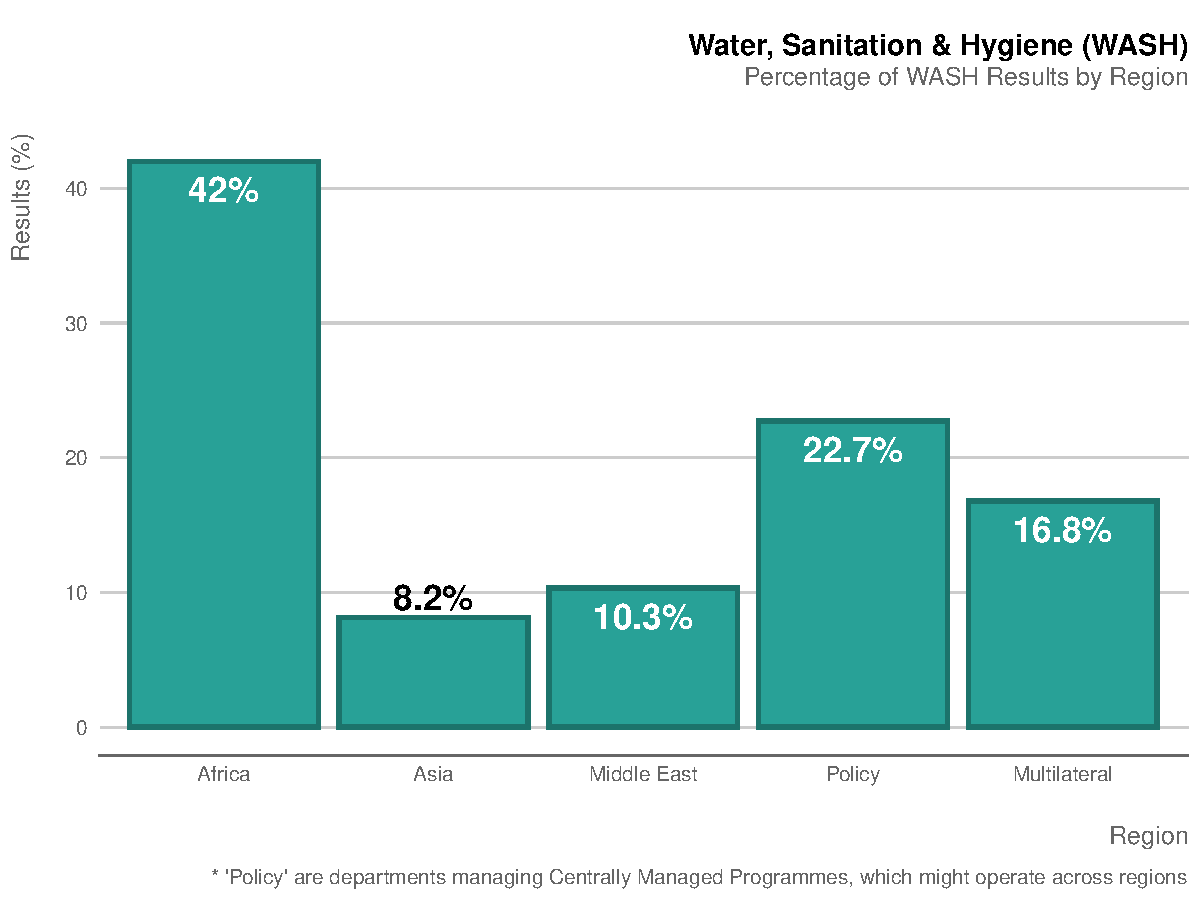
\includegraphics[width=0.8\textwidth]{../figs/wash_region_plot} \hfill
	\caption{Percentage of WASH results by region.}
	\label{fig:wash_region_plot}
\end{figure}


From 2015 to 2020, Africa was the largest beneficiary of DFID Water Supply, Sanitation and Hygiene (WASH) programmes, with 26.3 million beneficiaries reached. %
DFID also reached over 6 million beneficiaries in the Middle East --- the majority of whom were in Syria (4.9 million) --- and 5.1 million beneficiaries in Asia. %
A further 39\% (24.7 million beneficiaries) of DFID's WASH results were delivered via non-country specific programmes, non-region-specific programmes, and multilateral organisations. %

\begin{figure}[htbp]
	\centering
	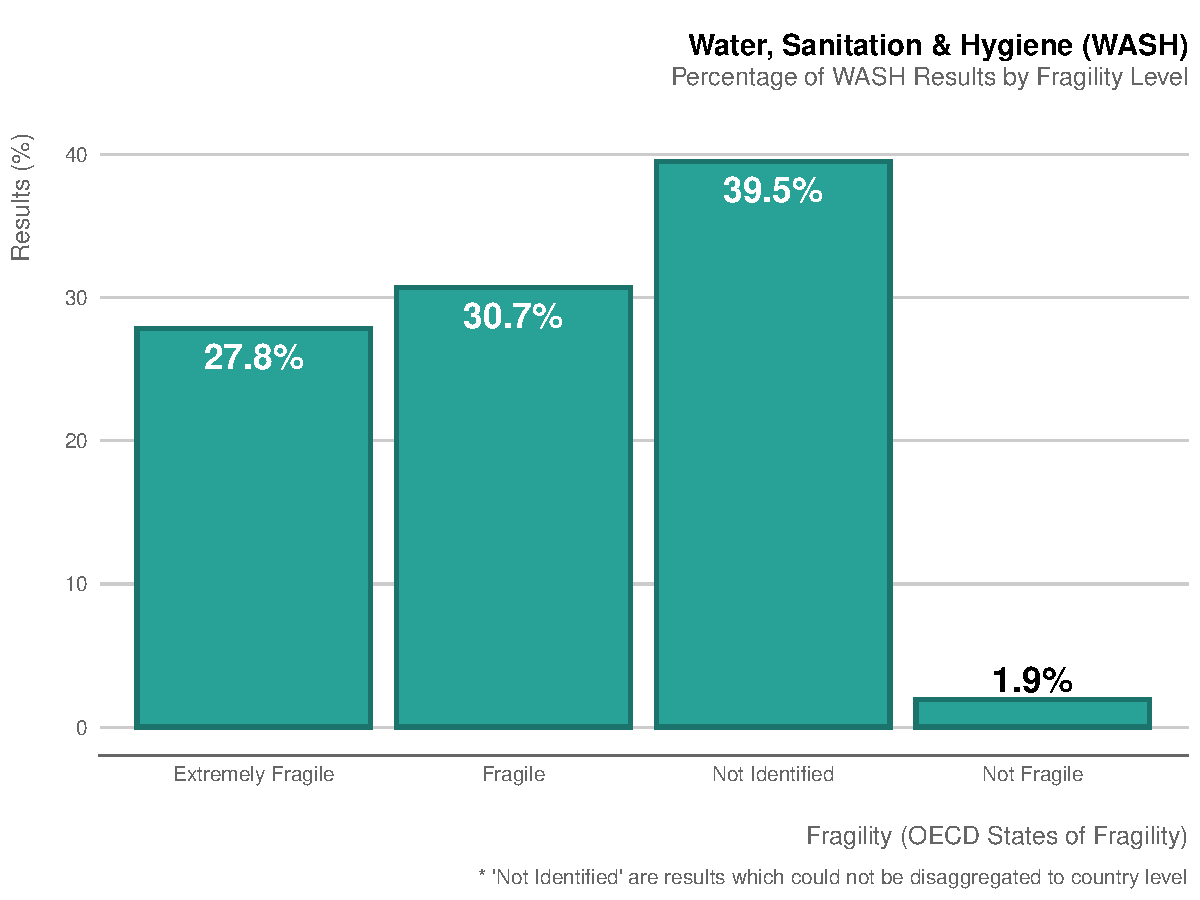
\includegraphics[width=0.8\textwidth]{../figs/wash_fragility_plot} \hfill
	\caption{Percentage of WASH results by fragility level.}
	\label{fig:wash_fragility_plot}
\end{figure}

DFID uses the OECD definition of fragile states, which is used to ensure we focus resources in the most fragile and conflict-affected countries. %
Most of the population reached by DFID WASH programs live in fragile states (37.8 million beneficiaries), including 17.4 million beneficiaries living in extremely fragile states. %

Of the results that have been disaggregated by gender from 2015 to 2020, DFID WASH programs reached 24.1 million women. %
In 2019/20 75\% of our reported WASH results were disaggregated by gender. %
This is a 4-percentage point increase in data disaggregation by gender between the results reported in 2018/19 and the results reported in 2019/20. %

\section{Context}
Successive governments have emphasised the importance of water supply and sanitation to support broader objectives for health, well-being and economic development. %
The November 2019 Conservative Party manifesto committed to build on existing efforts to end preventable deaths of mothers, new-borns and children  by 2030. %
Water supply, sanitation and hygiene are all necessary elements to secure the health outcomes that would meet this ambition. %
For example, safe water and sanitation is the most effective way of preventing 1,000 young children dying every day from diarrhoea. %

WASH is also critical in managing epidemic diarrhoeal diseases such as cholera as well as some of the most prevalent neglected tropical diseases, including trachoma, schistosomiasis and soil transmitted helminths. %

The provision of safe water, sanitation and hygiene is essential in protecting human health during the COVID-19 outbreak. %
We know the disease is highly infectious and can spread rapidly. %
Frequent and proper hand hygiene is therefore one the most important prevention measures for COVID-19 but requires sufficient availability of water. %

The non-health benefits of WASH are equally significant, especially for improving the lives of women and girls whose education and future prosperity can suffer from, for example, bearing the burden of collecting water. %

Based on 2016 data – the most recent available, 31\% of schools lack basic water supplies --- needed not only for drinking but also to keep toilets operating and to support hand hygiene and menstrual hygiene. %
Thirty-five percent of schools lack a basic sanitation service, and 900 million children worldwide go to schools without functional hygiene facilities. %
The situation undermines the quality of education received by girls, disempowering them, and many cases, keeps them out of schools. %

Other vulnerable groups can also benefit from improved water and sanitation, like the disabled and elderly people. %
As more people are provided with piped water at home it is easier for people with disabilities and their carers to be healthy and live in dignity. %

Investing in water and sanitation can represent good value for money. %
Globally for every \pounds 1 invested there is a return of over \pounds 4. %
In many countries, the returns are even higher. %
Improved WASH services, alongside investments to improve health, nutrition and education underpin just about every aspect of human and economic development. %

Sustainable Development Goal 6 aims to ensure availability and sustainable management of water and sanitation for all by 2030. It includes the targets:

\begin{adjustwidth}{0.5cm}{}
\textbf{Target 6.1:} By 2030, achieve universal and equitable access to safe and affordable drinking water for all.

\medskip

\noindent\textbf{Target 6.2:} By 2030, achieve access to adequate and equitable sanitation and hygiene for all and end open defecation, paying special attention to the needs of women and girls and those in vulnerable situations
\end{adjustwidth}

In 2019, the Joint Monitoring Program (JMP), supported by DFID, issued a progress report on household drinking water, sanitation and hygiene. %
This showed that in 2017, only 45\% of the global population had access to safely managed sanitation, with 71\% having access to a safely managed water supply. %
A further 29\% of the global population had access to a basic improved toilet and 19\% had access to at least a basic improved water supply. %

A second JMP report, also published in 2019, estimated that 26\% of all health care facilities lack a basic water supply; 21\% have no sanitation, and 16\% have no hygiene service. %
These failings undermine the promise of universal health coverage, adversely affect quality care and infection prevention and control and contribute to the unnecessary use of antibiotics and the spread of antimicrobial resistance. %

The cost of achieving the SDGs reflects the scale of their ambition. The World Bank has estimated that reaching the water and sanitation targets will require \$114 billion per year, excluding recurrent and replacement costs. %
Based on the current rate of progress, the JMP has estimated that only 1 in 5 of reporting countries is on track to achieve universal access to basic water by 2030. %
For sanitation the ratio is only 1 in 10. %
Meeting these ambitious targets will require much greater investment by countries themselves from both public finances and by attracting private capital investments. %

The UK has played a major role in helping poor people gain access to at least basic water and sanitation services, with over 64.5 million people benefiting from April 2011 to March 2015. %
We are now placing an increased emphasis on supporting countries to develop sustainable systems for water and sanitation service delivery. %

We have also helped establish key components of the global WASH architecture, including the Joint Monitoring Programme, and the Sanitation and Water for All partnership. %
We are leading the way in addressing climate change impact on water and sanitation services to ensure they are made more resilient to future threats. %

\newpage
